\documentclass[10pt]{beamer}

\usetheme{metropolis}
\usepackage{appendixnumberbeamer}
\usepackage[utf8]{inputenc}
\usepackage[russian,francais]{babel}
\usepackage{booktabs}
\usepackage[scale=2]{ccicons/ccicons}
\usepackage{pifont}
\usepackage{pgfplots}
\usepgfplotslibrary{dateplot}

\usepackage{xspace}
\newcommand{\themename}{\textbf{\textsc{metropolis}}\xspace}
%%\usepackage{polyglossia}
%%    \setdefaultlanguage{french} % main language
%%    \setotherlanguages{russian, hindi, greek, hebrew} % other languages 
%%\graphicspath{{images/}}	% Put all images in this directory. Avoids clutter.
%%\setmainfont{Latin Modern Roman}
%%\setsansfont{Latin Modern Sans}
%%\setmonofont{Latin Modern Mono}
%%\setmainfont[Ligatures=TeX]{Times New Roman}
%%\newfontfamily{\cyrillicfonttt}{Times New Roman}[Script=Cyrillic]

\usetheme{metropolis}
\usepackage{appendixnumberbeamer}
\usepackage[utf8]{inputenc}
\usepackage[russian,francais]{babel}
\usepackage{booktabs}
\usepackage[scale=2]{ccicons}
%\usepackage{xcolor}
\usepackage{wrapfig}
\usepackage{subcaption}
\usepackage{pgfplots}
\usepgfplotslibrary{dateplot}
\usepackage{graphicx}
\usepackage{xspace}
\usepackage{hyperref}
\usepackage{arydshln}
\usepackage{pifont}
\usepackage{enumitem}
\usepackage{xcolor}
%\usepackage{minted}
%%\usepackage{polyglossia}
%%    \setdefaultlanguage{french} % main language
%%    \setotherlanguages{russian, hindi, greek, hebrew} % other languages 
%%\graphicspath{{images/}}	% Put all images in this directory. Avoids clutter.
%%\setmainfont{Latin Modern Roman}
%%\setsansfont{Latin Modern Sans}
%%\setmonofont{Latin Modern Mono}
%%\setmainfont[Ligatures=TeX]{Times New Roman}
%%\newfontfamily{\cyrillicfonttt}{Times New Roman}[Script=Cyrillic]









\definecolor{greenperso}{RGB}{68,117,104}
\definecolor{greenblue}{RGB}{95,179,176}



\title{Programmation de Modèles Linguistiques 1, \\ L6SOPRG L3}
\subtitle{Crédits : Hugo Chevroton, CESR \& Angélique Allaire, ObTIC}
%\subtitle{A modern beamer theme}
\date{}
\author{Caroline Koudoro-Parfait\\ \quad {caroline.parfait@sorbonne-universite.fr\\}}
\institute{Observatoire des Textes des Idées et des Corpus - Obtic,\\ Sorbonne Center for Artificial Intelligence - SCAI,\\ Sens Textes Informatiques Histoire - STIH EA 4509, Sorbonne Université}
 \titlegraphic{\hfill
\includegraphics[height=.7cm]{images/sorbonne.png}}
\begin{document}
\maketitle

%\begin{frame}{Plan de la présentation}
%  \setbeamertemplate{section in toc}[sections numbered]
%  \tableofcontents[hideallsubsections]
%\end{frame}
\begin{frame}
  \frametitle{Généralités}
  \begin{block}{Organisation du semestre}
 \begin{itemize}
   \item CM + TD le Vendredi de 13h00 à 17h00 (C. Koudoro-Parfait \& LG Moreno Jimenez)
   \item Contrôle continu + projet + contrôle terminal
  
  \end{itemize}
  \end{block}
\begin{block}{Ressources}
  \begin{itemize}
  \item \href{http://paris-sorbonne.hosted.exlibrisgroup.com/F?func=find-c&ccl_term=idn=ppn199563403&local_base=MAH01}{TAL et Linguistique Informatique 1}, ISTE Ed. (Mohamed Z. Kurdi) 
  \item Speech and Language Processing (Dan Jurafsky), \url{https://web.stanford.edu/~jurafsky/slp3/} 
  \item Helpdesk : mail ou bureau 206/211 à Serpente (sur RDV)
  \end{itemize}
   \end{block}
\end{frame}

\begin{frame}
  \frametitle{Plan du cours}
\tableofcontents

\end{frame}
\section{Convertir un jupyter notebook en script .py}


\begin{frame}
 \frametitle{Étapes importantes}
\begin{itemize}

\item \textcolor{green}{\ding{51}} Commenter le code non essentiel 

\item \textcolor{green}{\ding{51}} Factoriser le code Jupyter Notebook en fonctions

\item \textcolor{green}{\ding{51}} Créer des scripts Python pour chaque tâches associées

\end{itemize} 
\end{frame}

\begin{frame}
 \frametitle{Étapes importantes}
\begin{itemize}
\item \textcolor{green}{\ding{51}} Commenter le code non essentiel : \# \\
\ding{220} les parties de programme qui ne \textbf{fonctionnent pas} ou \textbf{expérimentatoires}.

\pause

\item \textcolor{green}{\ding{51}} Factoriser le code Jupyter Notebook en fonctions. Observer votre notebook, n'y a t il pas :\\
\ding{220} des parties de code que vous répétez ?\\
\ding{220} des fonctions que vous répétez inutilement.

\pause

\item \textcolor{green}{\ding{51}} Créer des scripts Python pour des tâches associées.\\
\ding{220} Vous pouvez écrire un scripte initiale dans lequel vous appelez un autre script qui va contenir les fonctions que vous souhaitez utiliser
\end{itemize} 
\end{frame}


\begin{frame}
  \frametitle{Enregistrer le fichier au format python - .py}
  Dans la barre de tâche en haut de l'écran jupyter notebook :
  
  
  Aller dans Fichier \ding{219}  Télécharger au format \ding{219}  Python (.py)
  
  \begin{figure}
  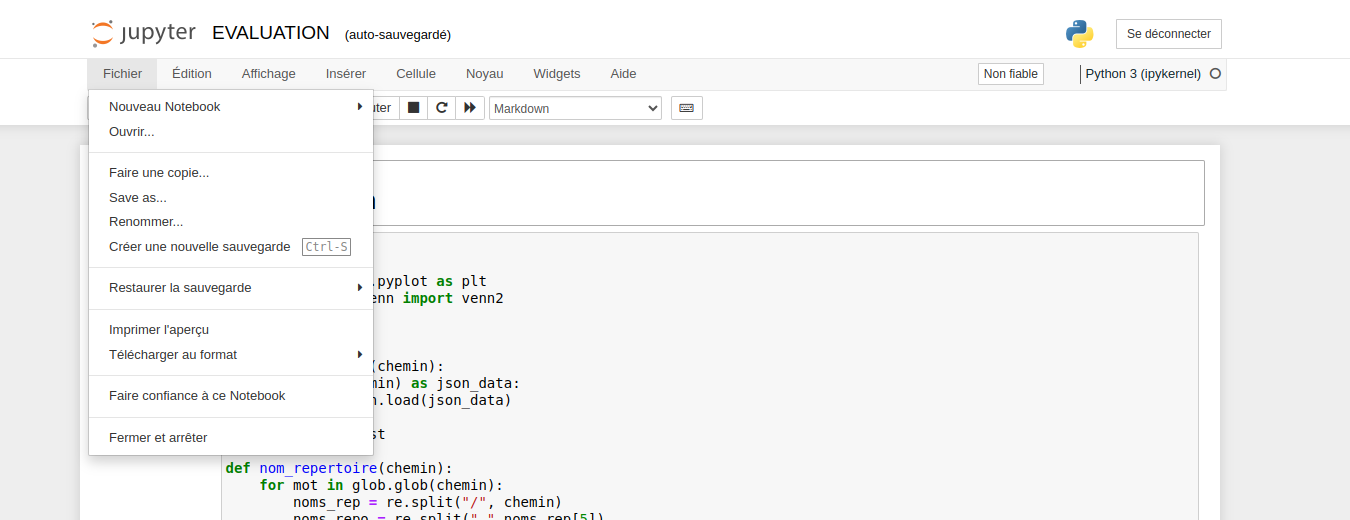
\includegraphics[width=10cm]{images/ynpb_convert_py.png}
  \end{figure}
 
\end{frame}



%\begin{frame}
%%  \frametitle{}
%  
%\end{frame}



\section{Spyder un autre environnement }  

\begin{frame} \frametitle{L'Éditeur 1}
  \begin{figure}
  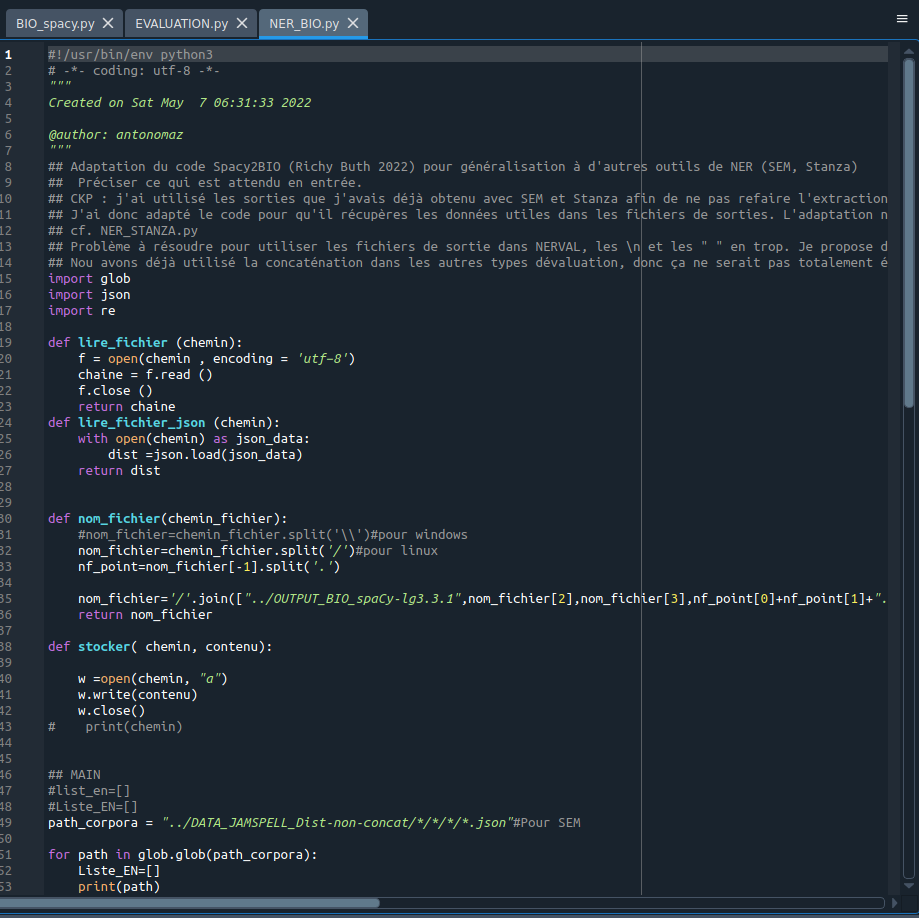
\includegraphics[width=7cm]{images/spyder_editor.png}
  \end{figure}
  
  \ding{220} +sieurs scripts peuvent être ouverts en même temps
\end{frame}

\begin{frame} \frametitle{L'Éditeur 2}

  \begin{figure}
  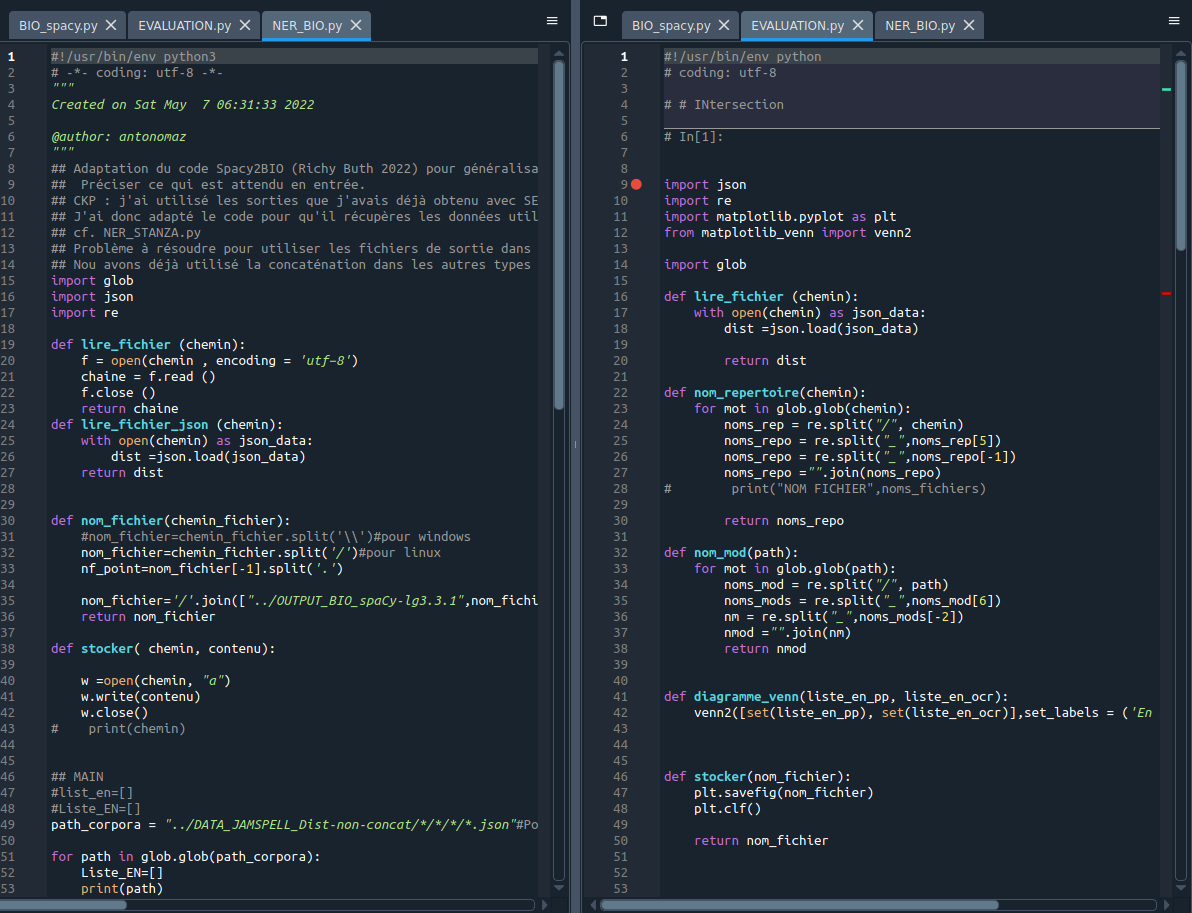
\includegraphics[width=7cm]{images/spyder_editor2.png}
  \end{figure}
  
  \ding{220} +sieurs scripts peuvent être ouverts côte à côte, ou l'un au dessus de l'autre.\\
  \ding{220} Cliquer sur
  \vspace{-0.3cm} 
  \begin{figure}
  
\includegraphics[width=0.5cm]{images/spyder_param.png}
  \end{figure} 
  \vspace{-0.3cm}
  et sélectionner \textit{split horizontally} ou \textit{split vertically}
\end{frame}

\begin{frame}  \frametitle{La console}
  \begin{figure}
  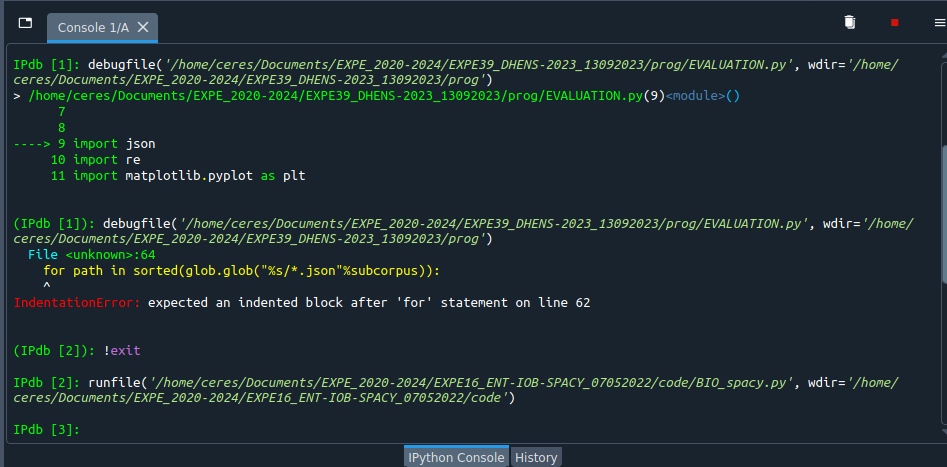
\includegraphics[width=10cm]{images/spyder_console.png}
  \end{figure}
  \ding{220} des lignes de codes peuvent être lancées depuis la console\\
  \ding{220} Les messages d'erreurs s'affichent dans la console \ding{219} Débogage\\
  \ding{220} Carré rouge en haut à droite de la console  == ordinateur calcul
\end{frame}

\begin{frame}
  \frametitle{Situer son script sur sa machine}
  \begin{figure}
  
\includegraphics[width=15cm]{images/spyder_chemin.png}
  \end{figure}
  \ding{220} Haut droite, fil d'Ariane : Indique où votre script est rangé sur la machine\\
  \ding{220} Haut gauche : permet de changer de dossier racine, d'explorer l'arborescence de votre machine
\end{frame}

\begin{frame}
  \frametitle{Renseignements sur l'environnement}
  \begin{figure}
  
\includegraphics[width=10cm]{images/spyder_infos.png}
  \end{figure}
  \ding{220} conda : base(3.11.5) \ding{219} Version de python utilisé dans l'environnement\\
  \ding{220} Completions: conda(base) \ding{219} Complétion automatique proposée\\
  \ding{220} LSP: Python \ding{219} Language Server Protocol (LSP) \\
  \ding{220} Line 24, Col 1 \ding{219} situation du curseur sur l'éditeur\\
  \ding{220}UTF-8 : Encodage\\
  \ding{220} LF \ding{219} File EOL status, Linux : LF, Windows : CRLF. Problème de fin de ligne par exemple.\\
  \ding{220} RW \ding{219} File permission \footnote{\url{https://www.warp.dev/terminus/linux-file-permissions-explained}}\\
  \ding{220}Mem 17\% \ding{219} Mémoire globale utilisée
  
\end{frame}

\begin{frame}  
\frametitle{L'explorateur de variable}
\begin{figure}
  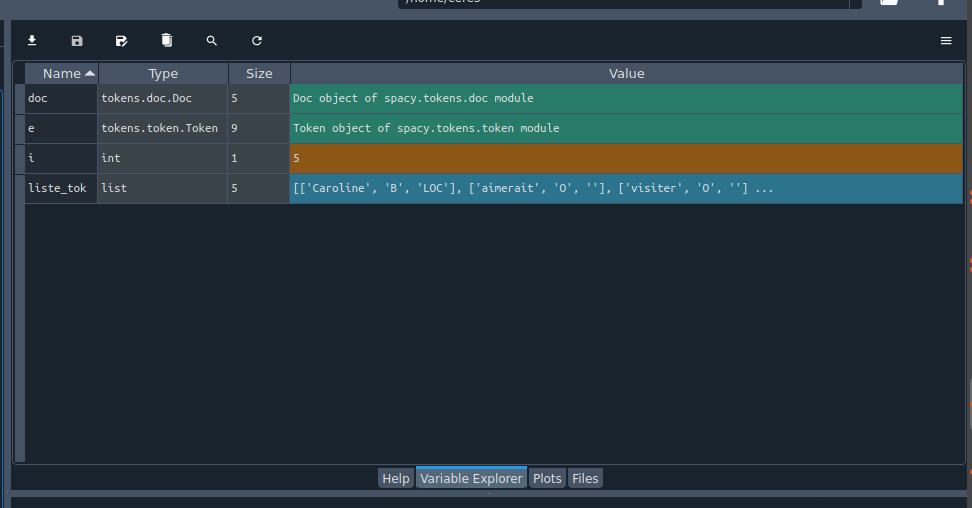
\includegraphics[width=10cm]{images/spyder_explo_variable.png}
  \end{figure}
  \ding{220} Accédez au nom de variable, type, longueur du contenu de la variable et valeurs
\end{frame}

\begin{frame}
  \frametitle{Sélectionner un fichier}
  \begin{figure}
  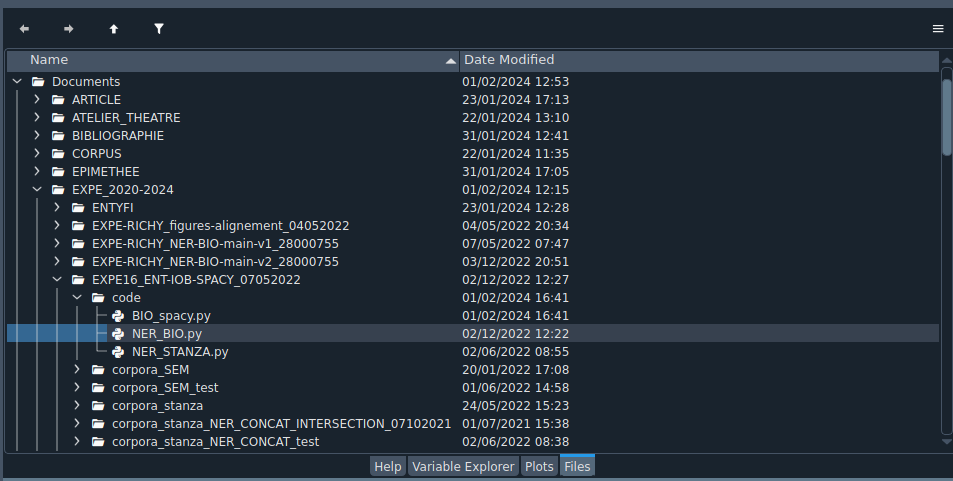
\includegraphics[width=9cm]{images/spyder_Files.png}
  \end{figure}
  \vspace{-0.3cm}
  Pour ouvrir un fichier vous pouvez :
  \begin{itemize}
  \item \ding{220} Sélectionner votre script dans l'explo. de fichier de votre machine et le déposer dans l'éditeur
  \item \ding{220} File \ding{219} Open \ding{219} Sélectionner votre script dans l'explo. de fichier affiché 
  \item \ding{220} dans l'explorateur onglet \ding{219} file \ding{219} naviguer \ding{219} double cliquer
  \end{itemize}
  \end{frame}

\begin{frame}
  \frametitle{Historique}
  \begin{figure}
  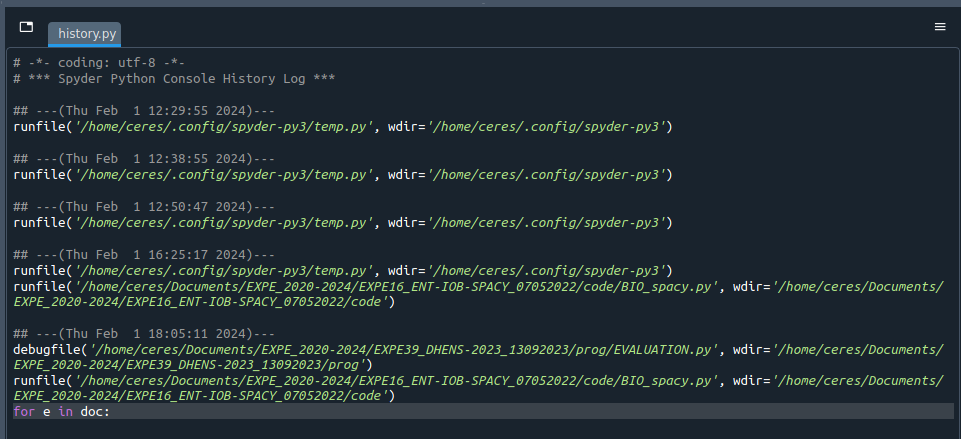
\includegraphics[width=10cm]{images/spyder_hystory}
	\end{figure} 
	\ding{220} Consulter l'historique des commandes  
  \end{frame}
  
\begin{frame}
  \frametitle{Débogage base}
  \begin{figure}
  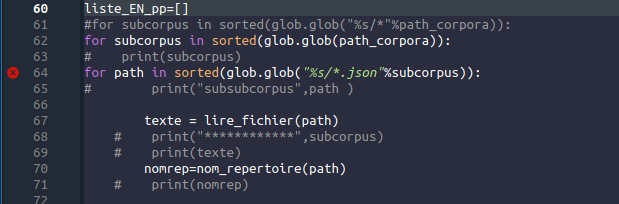
\includegraphics[width=10cm]{images/spyder_signal_erreur.png}
	\end{figure} 
	\ding{220} affiche qu'il y a un problème, passer la souris / cliquer dessus pour avoir le détail. 
  \end{frame}
  
\section{Listes, dico, set (et match !)}

\begin{frame}
  \frametitle{Petit point sur les listes}
  \ding{220} Une liste est une structure de données permettant d'accéder
à un objet par son index.\footnote{+ d'infos sur les listes \url{https://gayerie.dev/docs/python/python3/list.html}}\\


\ding{220} Pour illustrer :\\
\ding{80} supposons qu'une liste représente une rue.\\
\ding{80}Chaque habitant vit dans une maison avec un numéro.\\
\ding{80} Ce numéro est l'index de la liste grâce auquel on peut accéder
à l'habitant .


Syntaxe :
\begin{itemize}
\item* liste =[] :définition d'une liste vide
\item* liste =["Annie" , "Paul"] :défnition avec quelques éléments
\item* liste [0] vaut "Annie" , liste[1] vaut "Paul".
\end{itemize}



\end{frame}
\begin{frame}
  \frametitle{Petit point sur les dictionnaires}

\ding{220} Un dictionnaire est une structure de donnée permettant
d'accéder à un objet par une clef.\footnote{+ d'infos sur les dict. \url{https://gayerie.dev/docs/python/python3/dict.html}}\\
\ding{220} Dans un dictionnaire de langue, on utilise les mots
comme clef afin d'accéder à leur définition, qui sont ici
les objets.\\
\ding{220} Dans un dictionnaire, chaque \textbf{clef est unique}.\\
\ding{220} Par contre, \textbf{une même définition} peut correspondre à
\textbf{+sieurs clef}.
Syntaxe :
\begin{itemize}
\item* dico\_age =$\left\{\right\}$
\item* dico\_age =$\left\{ "Annie" : \textcolor{orange}{20} , "Paul" :18, "Antonia":  \textcolor{orange}{20} \right\}$
\item* dico\_age [ "Annie" ] vaut 20 .
\end{itemize}
\end{frame}

\begin{frame}
  \frametitle{Petit point sur les set - ensembles}
  \ding{220} c'est un groupement non ordonné d’éléments uniques \ding{220} pas de doublon.\\
  \ding{220} peut contenir des éléments de types différents.\\
  
  Syntaxe :
  
  \begin{itemize}
\item*  mon\_ensemble = set() != mon\_dico =$\left\{\right\}$
\item* fd
\item* gdfg
\item* gfdgfd
\end{itemize}
\end{frame}

\begin{frame}
%  \frametitle{}
  
\end{frame}







\documentclass[xcolor=table]{beamer}

\usetheme{metropolis}
\usepackage{appendixnumberbeamer}
\usepackage[utf8]{inputenc}
\usepackage[russian,francais]{babel}
\usepackage{booktabs}
\usepackage[scale=2]{ccicons}
%\usepackage{xcolor}
\usepackage{wrapfig}
\usepackage{subcaption}
\usepackage{pgfplots}
\usepgfplotslibrary{dateplot}
\usepackage{graphicx}
\usepackage{xspace}
\usepackage{hyperref}
\usepackage{arydshln}
\usepackage{pifont}
\usepackage{enumitem}
\usepackage{xcolor}
\usepackage{minted}
\newcommand{\themename}{\textbf{\textsc{metropolis}}\xspace}
%%\usepackage{polyglossia}
%%    \setdefaultlanguage{french} % main language
%%    \setotherlanguages{russian, hindi, greek, hebrew} % other languages 
%%\graphicspath{{images/}}	% Put all images in this directory. Avoids clutter.
%%\setmainfont{Latin Modern Roman}
%%\setsansfont{Latin Modern Sans}
%%\setmonofont{Latin Modern Mono}
%%\setmainfont[Ligatures=TeX]{Times New Roman}
%%\newfontfamily{\cyrillicfonttt}{Times New Roman}[Script=Cyrillic]

\title{Algorithmique et Programmation (TALA330A L3 INALCO)}
\subtitle{Crédits : Angélique Allaire, ObTIC}
%\subtitle{A modern beamer theme}
\date{17 octobre 2022}
\author{Caroline Koudoro-Parfait\\ \quad {caroline.parfait@sorbonne-universite.fr\\} \quad {}}
\institute{Observatoire des Textes des Idées et des Corpus - Obtic,\\ Sorbonne Center for Artificial Intelligence - SCAI,\\ Sens Textes Informatiques Histoire - STIH EA 4509, Sorbonne Université}
 \titlegraphic{\hfill
\includegraphics[height=.7cm]{images/inalco_logo.png}}




\begin{document}
\maketitle
\definecolor{greenperso}{RGB}{68,117,104}
\definecolor{greenblue}{RGB}{95,179,176}

\begin{frame}{Plan de la présentation}
  \setbeamertemplate{section in toc}[sections numbered]
  \tableofcontents[hideallsubsections]
\end{frame}

\section{Les Fonctions - Principe et généralités}

\begin{frame}{Les Fonctions - Principe et généralités}

\begin{itemize}[label=\textbullet, font= \color{greenperso}]
    \item Utiles pour réaliser plusieurs fois la même opération au sein d'un programme. 
    \item Elles rendent également le code plus lisible et plus clair en le fractionnant en blocs logiques.
\end{itemize}
\end{frame}


\begin{frame}{Les Fonctions natives Python}
    

Vous connaissez déjà certaines fonctions Python. Par exemple des fonctions internes à Python comme :

\begin{itemize}[label=\textbullet, font= \color{greenperso}]
    \item range() : indication pour effectuer une action un certain nombre de fois dans une boucle for
    \item len() : donner la taille d'une liste, d'une chaîne de caractères
    \item print() : affichage
    \item type() : type de la valeur 
\end{itemize}
\end{frame}



\begin{frame}{Les Fonctions}
Pour l'instant, une fonction est à vos yeux une sorte de « boîte noire » (voir figure 1) :
\begin{itemize}[label=\textbullet, font= \color{greenperso}]
    \item À laquelle vous indiquez aucune, une ou plusieurs variable(s) entre parenthèses. Ces variables sont appelées \textbf{arguments}. Il peut s'agir de n'importe quel type d'objet Python.

 \item Qui effectue une action.
\item Et qui renvoie un objet Python ou rien du tout.
\end{itemize}
\end{frame}


\begin{frame}{Les Fonctions}

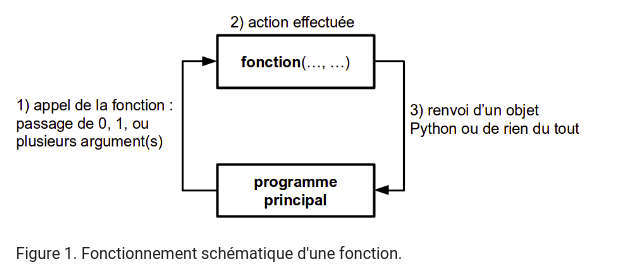
\includegraphics[scale=0.5]{images/fonctions.png}
    
\end{frame}

\section{Déclarer et appeler une fonction}

\begin{frame}{Les Fonctions}

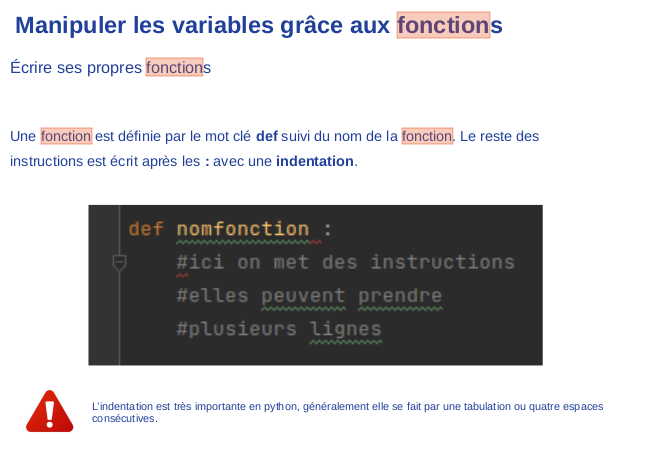
\includegraphics[scale=0.5]{images/fonction_2.png}
    
\end{frame}

\begin{frame}{Les Fonctions}

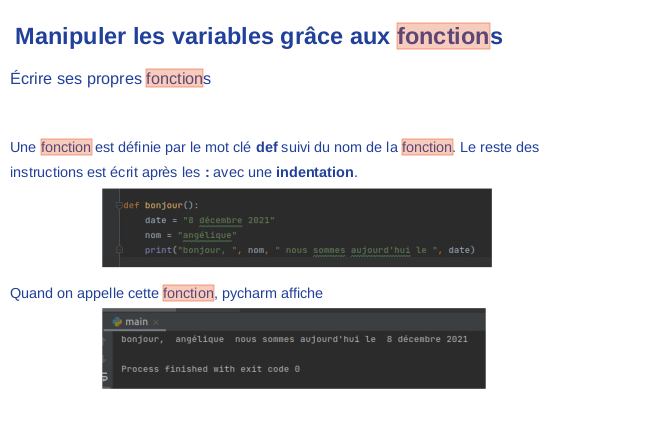
\includegraphics[scale=0.5]{images/fonctions_3.png}
\vspace{-0.3cm}
\footnotesize{$*$ \textit{pycharm} est un IDE, au même titre que \textit{Spyder ou Jupyter notebook}...}
    
\end{frame}

\begin{frame}{Les Fonctions}

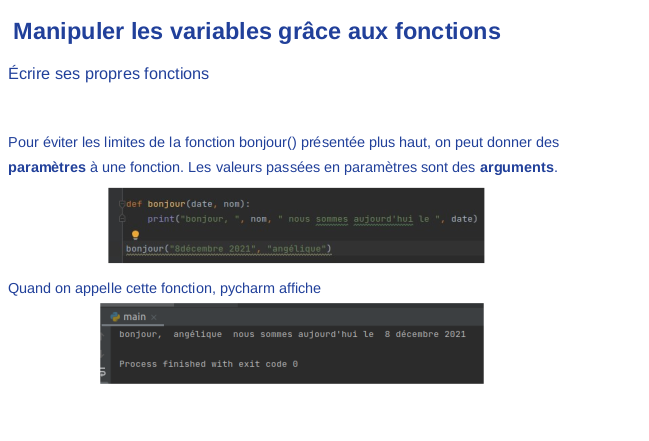
\includegraphics[scale=0.5]{images/fonction_3.png}
\vspace{-0.3cm}
\footnotesize{$*$ \textit{pycharm} est un IDE, au même titre que \textit{Spyder ou Jupyter notebook}...}
    
\end{frame}

\begin{frame}{Les Fonctions}

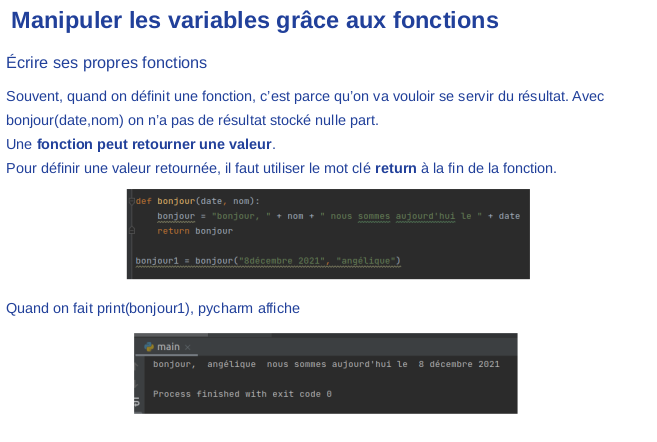
\includegraphics[scale=0.5]{images/fonction-4.png}
    
\end{frame}

\begin{frame}{Les Fonctions}

Exercice :
Écrire une fonction qui retourne l’endroit où nous sommes actuellement et ce que nous faisons en utilisant des paramètres
    
\end{frame}


\begin{frame}{Les Fonctions}
Ecrire la fonction 
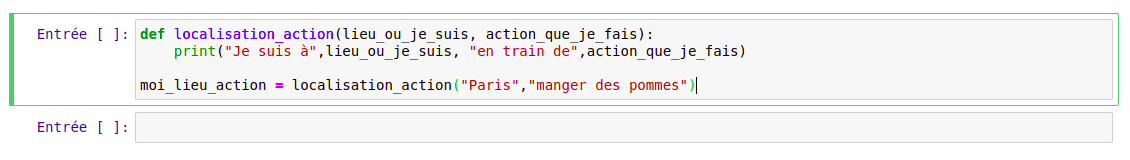
\includegraphics[scale=0.3]{images/fonction_1.png}
\pause

\vspace{1cm}
Quand on fait tourner le programme on obtient : 
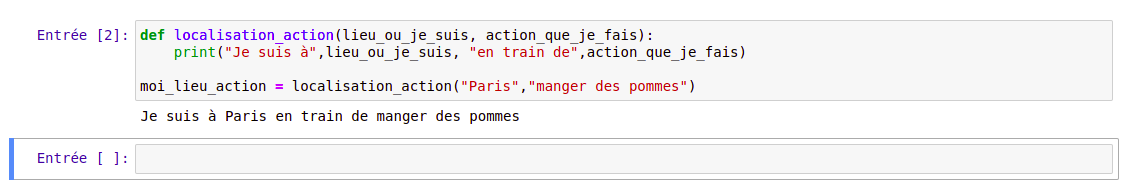
\includegraphics[scale=0.3]{images/fonction2.png}

\end{frame}
\end{document}

\end{document}
